\documentclass[a4paper,12pt]{article}
\usepackage{fullpage}
\usepackage{hyperref}
\usepackage{url}
\usepackage{graphicx}
%\usepackage{polski}
\usepackage[utf8]{inputenc}

\setlength{\parindent}{0pt}
\addtolength{\parskip}{\baselineskip}

\title{3rd Year Group Project\\Report Two\\\emph{Progress \& Revisions}}

\author{
    \small{Rafał Szymański}\\
  	\and
    \small{Maciek Albin}\\
    \and
    \small{Sam Wong}\\
    \and
    \small{Suhaib Sarmad}\\
		\and
		\small{Jamal Khan}\\
		\and
		\small{\{rs2909, mja108, sw2309, sss308, jzk09\}@doc.ic.ac.uk}
		\and
		\\Department of Computing - Imperial College London
}

\date{}

\begin{document} 
	\maketitle
	
	\section{Report I Amendments}
  After submitting our first report we realised the Iteration plan we proposed was flawed. 
%Original plan: 	
	% \begin{description}
	%   \item[First Iteration] MVP - basic news augmenting functionality and live updates.
	%     \begin{itemize}
	%       
	%       \item Setup DB and server to receive Tweets and RSS
	%       
	%       \begin{itemize}
	%         \item Research suitable DB (MongoDB)
	%         \item Select frameworks and architecture
	%         \item digging into twitter API \& RSS
	%       \end{itemize}
	%       
	%       \item Design algorithms to generate keywords (Look into using natural language processing libraries, there are a lot available for Python)
	%       \item UI Mockups and UX Research
	%       \item UI Implementation: Framework and plugins to use (eg jQuery, jQuery plugins, Twitter Bootstrap, etc)
	%       \item Getting the web app hosted
	%     \end{itemize}
	%     \item[Second Iteration] 
	%     Polished and Efficient implementation including Debugging, refactoring and optimisation
	%     \item[Third Iteration] 
	%     Extensions including:
	%       \begin{itemize}
	%         \item Sentiment Analysis algorithm
	%         \item Categorization algorithm    
	%       \end{itemize}
	%       
	%     \item[Fourth Iteration] 
	%     Final Product
	%   
	%   
	% \end{description}
	% 
	% \begin{itemize}
	% 	\item Week 1: Setup DB and server to receive Tweets and RSS, UI Mockups
	% 	\item Week 2: UI Implementation, Design algorithms to generate keywords
	% 	\item Week 3: Getting the web app online (Beta, Iteration 1)
	% 	\item Week 4: Debugging, refactoring and optimization (Iteration 2)
	% 	\item Week 5: Work on Extensions, Sentiment analysis algorithm, Categorization algorithm (Iteration 3)
	% 	\item Week 6: Final polishing of app (Iteration 4)
	% \end{itemize}
In many parts instead of focusing on the user facing features we have reported on the technical aspects of what we will do. One whole iteration was dedicated to ``Debugging, refactoring and optimisation''. That is not in the spirit of Agile Programming and, we believe, may incline the team to focus on less important things. With this in mind we've decided it would be very advisable if we revised our iteration plan rather quickly and followed that one, instead of the one submitted in Report One.

  We've also realised the product and feature descriptions given in the first report suffered from similar misconceptions. We all knew what we wanted to build, but when tasked with putting our thoughts on paper we again focused on less relevant technical details, rather then overarching user facing features.

  This section will detail the new iteration plan and describe what the project goals are in a more feature oriented manner. Bare in mind this is the iteration timeline and feature list we've agreed on soon after submitting the first report and there have been some changes to this detailed in the \emph{Progress} section. 

  \subsection{Project Description and Key Requirements}
  In this project we want to create a website that will allow people to see an aggregated public Twitter reaction to top news stories emerging around the world. We want people to be able to glance at our UI, se what's happening right now and what are the dominant trends on Twitter related to that story.

  The key requirements of our project are:
  \begin{itemize}
   \item Displaying top news stories from Google News
   \item Displaying relevant most influential tweets next to the stories
   \item Displaying aggregated wordclouds next to the stories. This means analysing which words appear most often with relation to the news story.
   \item The UI needs to be fluid and updating in real-time and on its own - the user should not be forced to hit a refresh button at all. It should also be fun to look at.
  \end{itemize}

  The extensions we want to implement are:
  \begin{itemize}
   \item Attaching pictures related to the news story. These would be aggregated from Twitter and news articles.
   \item Attaching a general category to news stories (art, politics, etc.). This would be based on the tweets related to the story, not the story itself. We want to know what people think the news is about, not what news editors tell them.
   \item Displaying the general approval of the story. We can measure whether a tweet is positive or negative towards the topic (this is called \emph{sentiment analysis}) and we want to use these measurements to tell users whether the reaction to the news story is positive or negative.
  \end{itemize}

  \subsection{Iteration Details and Timeline}
  This iteration timeline starts at the week of our initial report. Previous weeks were utilised to decide on the goals of our project and coordinate with our project supervisor.
  \begin{description}
   \item[Iteration 1] \emph{Weeks 4-5}\\
   This iteration will also require us to do all of the initial setup. Find a way to fetch tweets relevant to news stories, etc. Hence the longer time period required.
   \begin{itemize}
     \item First attempt at the UI. It will be polished and new features will be added throughout iterations.
     \item Display current news stories.
     \item Generate keywords from news stories and fetch relevant tweets. This is a necessary part of the entire system.
   \end{itemize}
   \item[Iteration 2] \emph{Week 6}
   \begin{itemize}
     \item Wordclouds generated from tweets related to news stories.
     \item Influential tweets related to news stories.
   \end{itemize}
   \item[Iteration 3] \emph{Week 7}
   \begin{itemize}
     \item Add the ability to analyse whether the tweets are positive or negative and present the aggregated result in the UI.
   \end{itemize}
   \item[Iteration 4] \emph{Week 8}
   \begin{itemize}
     \item Categorise tweets and based on these categories categorise the news stories themselves. Add that to UI.
   \end{itemize}
   \item[Iteration 5] \emph{Week 9}
   \begin{itemize}
     \item Fetch pictures relevant to news stories and present them in the UI.
   \end{itemize}
   \item[Iteration 6] \emph{Week 10}
   \begin{itemize}
     \item Final application polish and validating if everything is \textbf{really really} working before final submission.
   \end{itemize}
  \end{description}

	To measure our velocity, we decided to use burn down charts, which you can see in the next section on \emph{Progress}.
	
	\section{Progress}
	We are at the end of week three of the iteration schedule. We are more or less on schedule but our iteration plan needed some changes. We'll talk about the revised iteration plan in the next section, for now let's focus on what we've accomplished and what problems we have had.
	
	\subsection{Iteration 1}
	We have completed this iteration, but some parts of it were finished long after the other parts. To start with we had to do all of initial setup (continuos integration, basic database, deciding on and writing the basic architecture), which took us about a week to complete and we consider that part a success.
	
	One of the decisions we've made was to have the analysis part and the UI part of the application as separate as possible. We still think it was a good decision (it is going to make extending the application much easier), but it created a bit of a disconnect between the team responsible for the backend and the frontend team. We believe that this caused us to put off connecting the UI to the API and the API to the database for too long. It ended up being a part of the second iteration and there were some unforeseen problems that meant we had to put off implementing top tweets in the UI for later. The UI and the analysis were good on their own, but connecting them together proved to be more difficult. Nevertheless, as described later, we now have a production server, where the changes go live right after each git push.
	% Mention we have set up our private git repo? From report1:
	% We will be using git for version control. Currently the project is hosted on github\footnote{\url{https://github.com/radicality/Twitter-News}}, but we will probably move it soon to our own VPS to set up continuos integration, and instant deployment.
	
	%	'Failure to develop keyword algorithm in time' was a potential risk
	The other problem we've encountered was of a technical nature. We tried to design our own keyword generator, but it turned out to be challenging and started to take quite a lot of time. In report one, we said ``Failure to develop keyword algorithm in time was a potential risk''. Since generating keywords was not a goal of our project we decided to use an external API\footnote{\url{http://www.alchemyapi.com/}} to perform that task. It works, but unfortunately the quality of keywords is quite low (we get keywords such as \emph{video}, or \emph{news} which make for a lot of irrelevant tweets). We provisionally added improving the keyword generation as part of one of the next iterations.
	
	We've also implicitly assumed that the UI should be live updating from the start. This is not the case right now however, as we've realised implementing it would take a lot of valuable time and we pushed that forward in our revised schedule. Burn down chart for this iteration is visible in Figure~\ref{burndown1}. According to it we haven;t been able to complete all the features in this iteration. Most of it due to some unforeseen technical difficulties and some people management issues. We talk about those in more detail in \emph{People Management}. Due to these problems we pushed some of the development to next iteration.
	\begin{figure}
	  \begin{center}
	  \caption{\label{burndown1} Burn Down Chart for Iteration 1}
		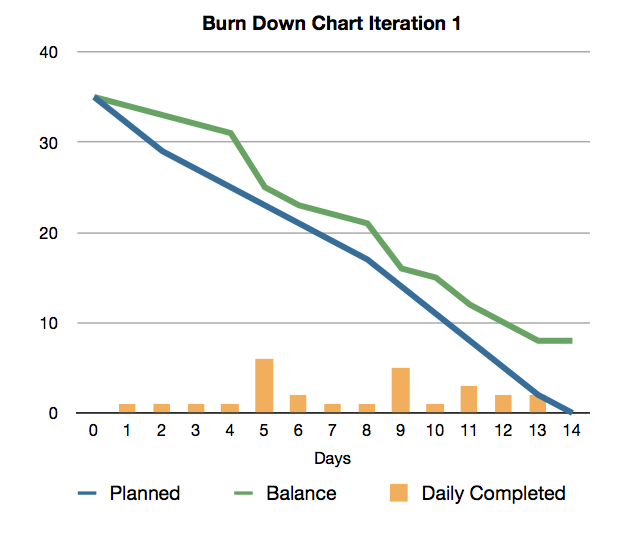
\includegraphics[scale=0.4]{burndown1.png}
    \end{center}
	\end{figure}
	
	\subsection{Iteration 2}
	Most of the iteration has been completed. Wordclouds are being generated and displayed in the UI, and we have the backend part done for displaying top tweets. Unfortunately for reasons outlined in the previous section we have not been able to implement the UI part responsible for displaying them. Part of the integration between the UI and the backend analysis thread has been moved here and has been completed. Burn down chart for this iteration is visible in Figure~\ref{burndown2}. This shows we again had some problems with finishing all the features. We think the main reasons for that are the problems we had with \emph{People Management} which we outline in the appropriate section. We believe these will be fixed and next iteration should be right on track.
	\begin{figure}
	  \begin{center}
	    \caption{\label{burndown2} Burn Down Chart for Iteration 2}
		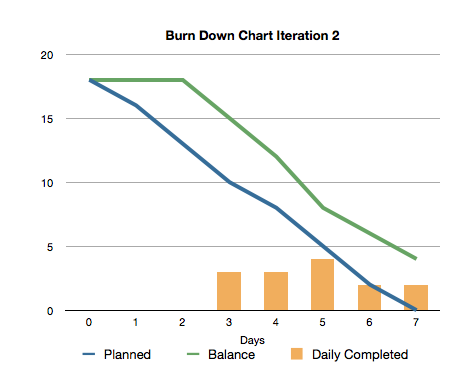
\includegraphics[scale=0.6]{burndown2.png}
	  \end{center}
	\end{figure}
	
	\subsection{Iteration 5}
	When developing the UI we've realised how easy it was to attach relevant pictures to news stories. We've managed to incorporate that into the work done during Iteration 2, and moved it out of Iteration 5 in the revised schedule. 
	
	\subsection{Current Product}
	
	We have achieved quite a bit both infrastructure wise and user-visible-features wise.
	
	\subsubsection{User Visible Features and UI}
	
	Here is a picture of what our current UI - the user deliverable product - looks like:
	
	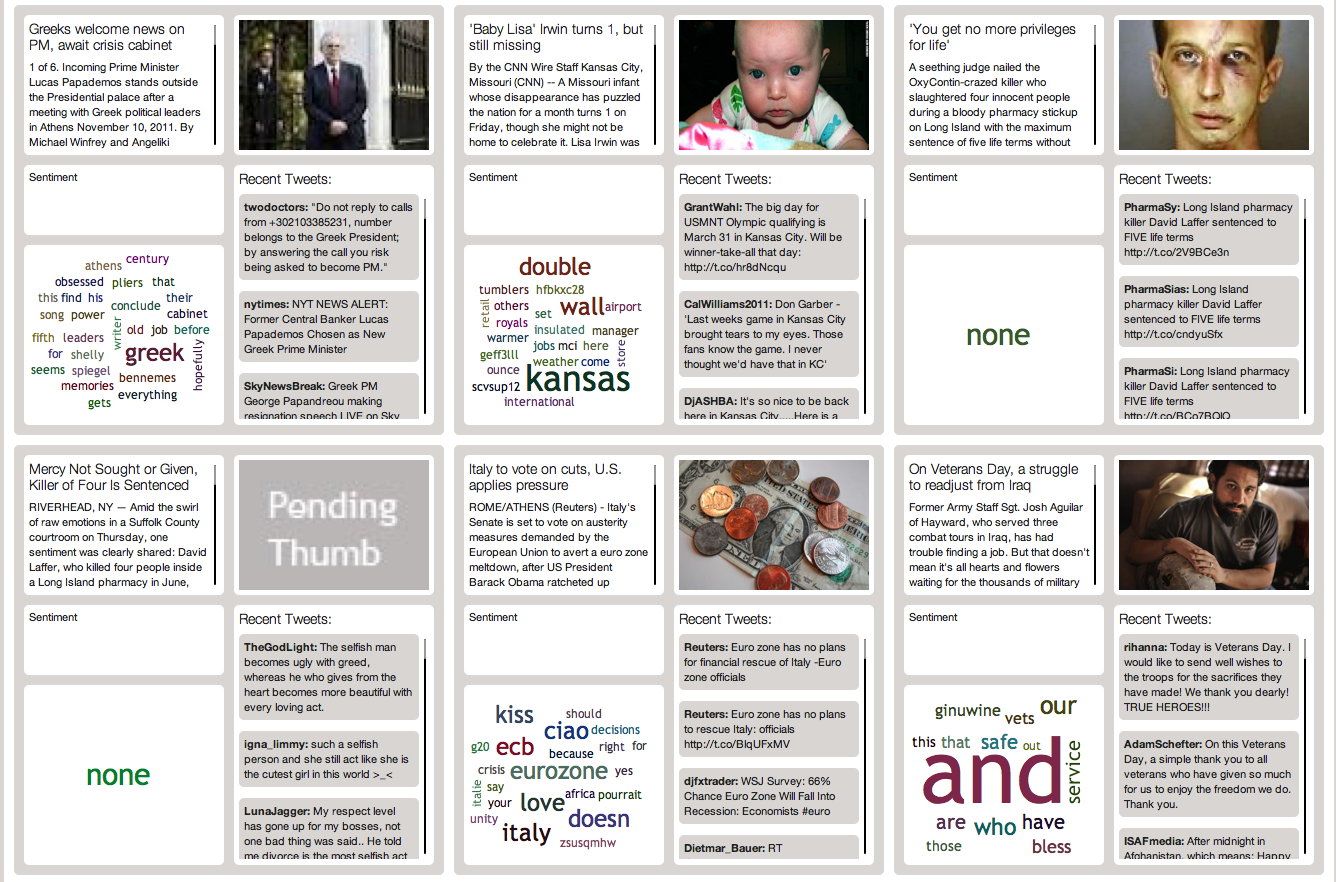
\includegraphics[scale=0.36]{website.png}
	
	This is a user visible feature, and we are happy that we have reached a state that connected the frontend and the backend, and created visible features.
	
	\subsection{Infrastructure accomplishments}
	
	We have accomplished a number of things infrastructure wise too. Apart from the things detailed in the iteration plan, such as constructing word clouds in the backend, we have set up a proper production environment at \url{http://twitter.rafal.io}\footnote{This will constantly be changing, and hence may break at times}.
	
	Whenever a code push occurs to our git repository, we have a git post-receive hook that copies the static files appropriately, and restarts the uwsgi process\footnote{This is the process that serves the python code}. This means that as soon as a code push occurs, the new version is live.
 
	Infrastructure-wise, on the outer layer resides Nginx, which proxies requests to the lower level uwsgi process that serves the api and the main page. Static content, such as javascript files or images, are directly handled by Nginx.
	
	  Other than internal things to help us work with the project, there have been no infrastructural changes. We are still using a Python backend, a JavaScript (jQuery) front end and a python web framework called Flask to provide API for our UI. For data storage, we are using MongoDB, which proving very useful and easy to use. After deploying and running the application for a couple of hours, we noticed rather high disk IO - we are planning to look over this and see how we can restructure our database queries, or lower their complexity, in order to reduce disk IO. For testing, we are using our personal computers.
	  
	  This is an information flow diagram that shows a high level view of our entire system:
	  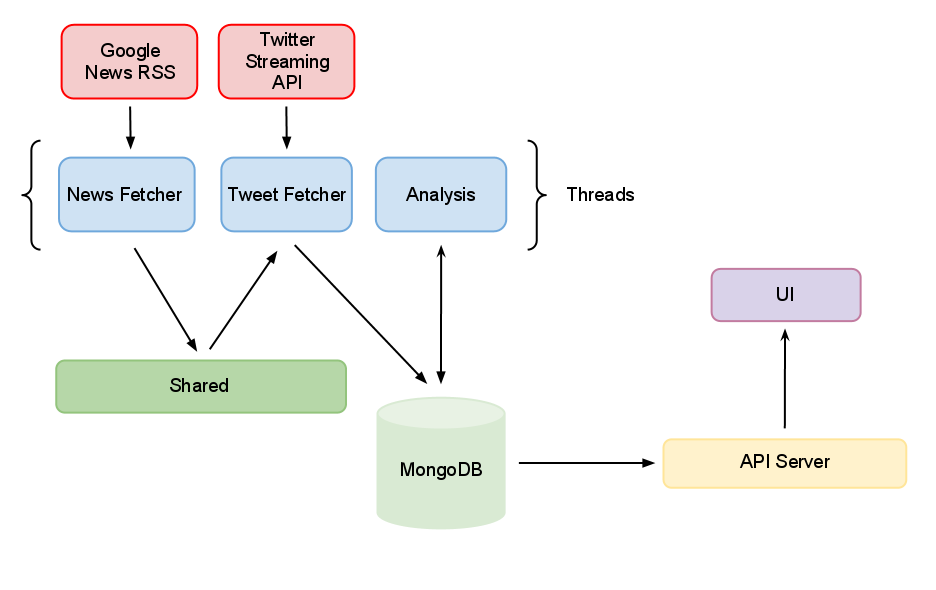
\includegraphics[scale=0.5]{infrastructure.png}
	
	\section{Revisions}
	
	\subsection{Revised schedule}
	
	\begin{description}
   \item[Iteration 3] \emph{Week 7}
   \begin{itemize}
     \item Add the ability to analyse whether the tweets are positive or negative and present the aggregated result in the UI.
     \item Display most influential tweets relevant to the story.
   \end{itemize}
   \item[Iteration 4] \emph{Week 8}
   \begin{itemize}
     \item Categorise tweets and based on these categories categorise the news stories themselves. Add that to UI.
     \item Improve keyword generation and thus the relevancy of information displayed to the end user.
   \end{itemize}
   \item[Iteration 5] \emph{Week 9}
   \begin{itemize}
     \item Make the UI update on it's without the need to refresh the browser.
   \end{itemize}
   \item[Iteration 6] \emph{Week 10}
   \begin{itemize}
     \item Final application polish and validating if everything is \textbf{really really} working before final submission.
   \end{itemize}
  \end{description}
  
  \subsection{Notes on the revised schedule}
	
	Neither our key requirements, nor the extensions have changed.
	
	%	FYI only... from report1,
	%	We have decided to use Python as the core programming language, along with MongoDB as the persistent datastore for keeping news and tweet information. MongoDB is particularly useful, as it allows easy saving and retrieval of tweets that come in json format and as opposed to a rigid SQL database it allows us to store `documents'. For the UI we'll be using HTML5 and JavaScript.
  
	In our previous report, we failed to realise that progress should be measured by user-visible features, instead of things like backend work that doesn't bring user-visible usable features. We now think our progress should be measured by visible results to the end user. As our project is web based, these results would include seeing news stories on a web page along with relevant tweets. Nevertheless, our progress with user visible features has been rather slow as we have concentrated more on the backend, which is not a user visible feature.

	From now on, we will strive to concentrate on the holistic effort, and make sure new and working user visible features are frequent.
	
	\subsection{Testing}
	%	We said we are using PyUnit, is that still true?
	%	We will be using a unit testing framework to check that the code we are writing meets its specification. This will be done using the PyUnit\footnote{\url{http://pyunit.sourceforge.net/}} testing framework.
	
	In the previous report we wanted to use unit tests as a primary way of testing various functional parts of the project. After looking over the project again, and having a discussion about testing during the Software Engineering Methods tutorial session, we realized that testing our product will be harder than expected.
	
	Our frontend is very light, and currently consists just of one page that's filled and structured with the data we have pulled using our API. There currently isn't any user interaction, so using testing frameworks such as Selenium can't be done yet. It is in our plan to have user features, such as clicking on a story and seeing more detailed information about it. Now, that will be easily testable using Selenium.
	
	Since our site consists of downloading, analysing, and displaying live data, it is not particularly simple or easy to write tests for this. Just like we wrote in report one, we are still planning on using pyunit. Our strategy now is to set up dummy data for which we know what data we want to get back, and then test whether the API returns the correct JSON output we require. After doing API testing, we will set up Selenium test that check whether that data is indeed being loaded onto the page.
	
	\section{People Management}
	
	As it often happens with group projects, problems relating group interactions and dynamics surface. Firstly, in our group, everyone knows each other well and is good friends with everyone else, which reduces the authoritative attitude of any one group member towards others. In a real life project, you have a manager with an authoritative position to do things such as lay you off, which certainly induces at least a little bit of motivation. In a university project where all the members are good friends, it is harder to establish an authority that is able to motivate others, especially during a time where everyone has a lot of other personal tasks at hand; motivation has to come from within the group members.
	
	During this term all of us have lot of other personal responsibilities, including a lot of coursework for other subjects, setting up and studying for internship interviews for next year, and teaching PMT classes, among many others. Considering every one of us has so many personal tasks that directly affect just him and not the group, we are seeing decreased motivation towards the project from all group members. We are directly experiencing \emph{Social Loafing}\footnote{\url{http://en.wikipedia.org/wiki/Social_loafing}}, which is ``the phenomenon of people exerting less effort to achieve a goal when they work in a group than when they work alone.'' It still seems that we are having problems keeping to the iteration task assignment on Trello\footnote{\url{http://trello.com}}, ie we are not completing the iteration subtasks within the timeline. The root cause of this is mostly likely related to the above explained \emph{social loathing}, and diffusion of responsibility within a group without a clear authoritative figure.
	
	%The first line is... erm....
	Our current proposed solution is rationalising to everyone the relative importance of this project compared to all other coursework - $440/1700$ points. Receiving a \textbf{C} for our first report was disappointing and a blow to our motivation, as none of us had gotten a C in Imperial before, but on the other hand it was a sign we need increase the quality of our work and approach the project more seriously.
	
	% Quotable stuff from report1
	% For development itself we will try to utilise \emph{paired programming} as much as possible. We believe this will allow all members of the team to understand major parts of the application in detail and help to even out different levels of expertise between team members. We also believe it will boost the team's productivity.
	We have separated our group of five people as follows: 2 for UI, and 3 for backend, so everyone is doing what they are more comfortable with. Both of these subteams do pair programming. Many times one of us knows something useful, for example a specific MongoDB query syntax, and can help the other without having to resolve to Google. This ensures a good flow of information between the team, and levels out our knowledge. Nevertheless, what we still thrive to have is a \emph{bus count}\footnote{\url{bit.ly/j1zquA} - quite interesting article.}\footnote{Bus count - ``how many people in your team have to get hit by a bus before you’re all dead in the water''} of the size of our group - we want everyone to understand, and if needed, to work on any part of our stack. This development technique follows with what we stated in report 1 - ``For development itself we will try to utilise \emph{paired programming} as much as possible. We believe this will allow all members of the team to understand major parts of the application in detail and help to even out different levels of expertise between team members. We also believe it will boost the team's productivity.''
	
	% Quotable stuff from report1

	We try to establish fair contribution by everyone by assigning to everyone tasks on Trello. In report 1 we said \emph{We shall have scrum meetings either daily, or every two days, where we will discuss the progress of the task everyone has been assigned to for that week. We aim to successfully complete the required tasks at the end of each iteration period.} We have planned to have frequent scrum meetings regarding the completion of tasks, but instead, since we all see each other during lectures anyways, we usually discuss the progress without having a dedicated meeting. What we need to do is actually get into the habit of having a dedicated progress meeting more frequently, where everyone has to showcase what they achieved in the previous 2 or 3 days.
	
	\section{Ethical and Environmental Impact}	
	
	The ethical issues we have thought about addressing are as follows:
	
	\begin{itemize}
	  
	  \item All technologies that we are using are open source. Python has an OSI-approved license\footnote{\url {http://docs.python.org/license.html}}, our server is written using Flask which is BSD Licenced\footnote{\url{http://flask.pocoo.org/docs/license/}} and MongoDB is also open source\footnote{\url{http://www.mongodb.org/display/DOCS/Licensing}}. The server is the widely used Nginx, which has a BSD-like license.
	  
		\item We are storing tweets, which are not our property. We copy the whole tweet to our database, which originally is the property of the original author and of Twitter. This is not exactly a compromising situation, but it nevertheless should be considered from an ethical standpoint.
		
		\item We are possibly aggregating information and presenting it in such a fashion that could reveal new and interesting patterns - patterns that might be surprising or ones that others don't agree with. We would also probably need to state that the results are merely the results of our algorithmic analysis, and not our personal viewpoint regarding the current news story.
		
		\item In addition, the news stories we are aggregating from Google News may be biased as it is based on what Google believes to be the top stories, and other peoples point of view as to what news is top may differ around the world.
		
		%'Small amount of tweets for a news story' & 'DB grows too quickly / run out of space / efficiency problems.' were potential risks in report1
		\item Our project currently only works for just top 10 stories from google news, and the volume of tweets is already quite high (can be as high as 50 a second). This means that the database is growing large quite quickly. If this project were to be extended to support many more news services, it would have to be distributed over more machines, along with more database instances to support the larger volume of data. This would be something to consider if machines or EC2 instances were to be bought. Already, after running the product over the night, there was a notification from the VPS provider notifying about high disk IO rate. These type of problems could be classified as an environmental issues. 
	  
	  
  \end{itemize}
  

\end{document}